%!TEX root = ../main.tex

\chapter{基于锚节点的论坛帖子抽取}

\section{概述}
\label{sec:pean-intro}

随着互联网技术的快速发展,我们已经进入Web 2.0的时代\citeup{o2007web}。
不同于早期Web 1.0的网络应用,Web 2.0更强调用户生成内容(User-Generated Content,UGC),
可用性和互操作性,开始以用户为中心,体现资源平等的特点。
用户能够在社交网络中相互交流和协作,越来越多的人向虚拟社区贡献着自己产生的内容,
不同的观点和意见在这里交融碰撞,而不是在早期网站上那样被动地接收有限的内容。
网络论坛就是Web 2.0中的典型代表,用户可以在论坛上发帖、回帖进行讨论,
是一种交互性强、内容丰富而及时的网络应用。

一个典型的网络论坛组织结构如图~\ref{fig:forum-structure}~所示,
论坛一般按照话题分为若干个板块(Board);
板块内部用户围绕具体事件进行的一系列发帖、回帖统称为Thread,一般按照发帖时间线性排列;
在一个Thread内部,用户的每一次发帖是Post。
以网易论坛\footnote{http://bbs.163.com/}的一篇帖子为例,如图~\ref{fig:forum}~所示,
红色实线圈出的是每一个Post,它们按照时间顺序排列,
包含发帖人、发帖时间、发帖内容等元信息,共同组成了一篇帖子的核心内容。

\begin{figure}[htbp]
\centering
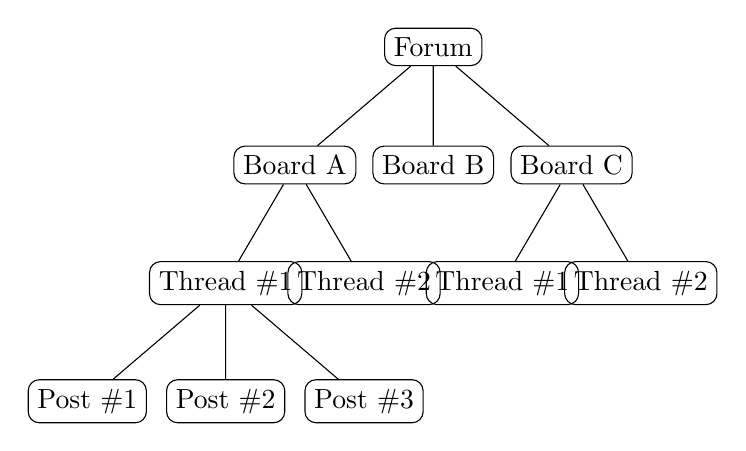
\begin{tikzpicture}[
sibling distance=5em,
every node/.style={rectangle,rounded corners,draw},
]
\node{Forum}
  child{node{Board A}
    child{node{Thread \#1}
      child{node{Post \#1}}
      child{node{Post \#2}}
      child{node{Post \#3}}
    }
    child{node{Thread \#2}}
  }
  child{node{Board B}}
  child{node{Board C}
    child{node{Thread \#1}}
    child{node{Thread \#2}}
  }
;
\end{tikzpicture}
\caption{论坛典型结构}
\label{fig:forum-structure}
\end{figure}

\begin{figure}[htbp]
\centering
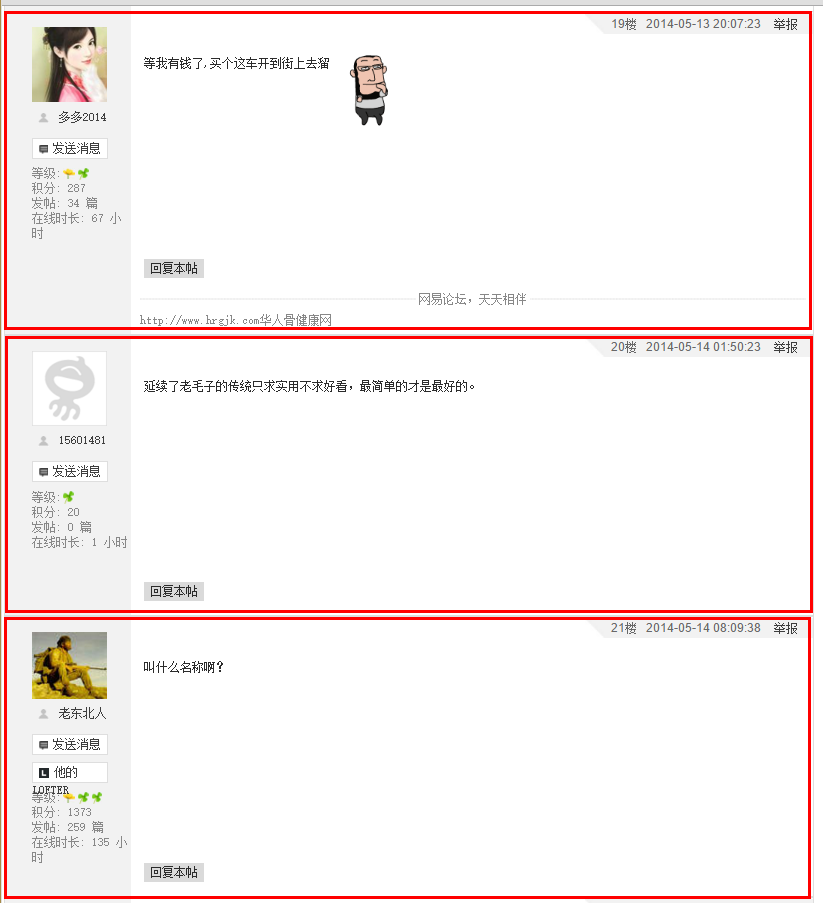
\includegraphics[width=0.9\textwidth,height=0.45\textheight]{forum}
\caption{论坛帖子实例}
\label{fig:forum}
\end{figure}

由于HTML网页所固有的半结构性,被设计为用户能够方便阅读,却不能被机器有效读取的形式。
虽然用户能够很容易区分不同的帖子,但面对结构样式各异的论坛网站,
如何从论坛网页中自动化地抽取帖子,转化为结构化的数据,
是一个很有挑战性的工作,也是舆情爬虫系统的重要环节。

本章利用论坛帖子中普遍存在的发帖时间信息作为锚节点,
提出一种基于锚节点的帖子抽取方法。
~\ref{sec:cevc-other}~节简单介绍对比算法MiBAT(基于锚点树的数据记录抽取算法)
的原理和实现细节;
~\ref{sec:pean-method}~节详述本文提出的基于锚节点的论坛帖子抽取算法PEAN
(Post Extraction via Anchor Nodes);
~\ref{sec:pean-experiment}~节进行论坛帖子抽取实验,并分析实验结果;
~\ref{sec:pean-conclusion}~节总结本章。

\section{对比算法及实现}
\label{sec:pean-other}

本章的对比算法为MiBAT\citeup{song2010automatic}
(\textbf{Mi}ning data records 
\textbf{B}ased on \textbf{A}nchor \textbf{T}rees),
基于锚点树的数据记录抽取算法。

面对论坛帖子中UGC内容格式自由、复杂多变而干扰相似度计算的问题
(图~\ref{fig:post-match}~),MiBAT的主要解决方法是,
在树相似度计算过程中,尽可能选择隶属于格式化模板的一部分节点进行比较,
而不是将所有节点全部考虑进去。
这里相互比较的节点子集,称为tree fragments。
树相似度定义扩展为:

\begin{definition}
\label{def:tree-ex-sim}
已知$M$是两个树$T_1$和$T_2$的匹配,$f$是tree fragment选择函数,
则$T_1$和$T_2$在$f$作用下的相似度是:
\begin{equation}
TreeSim_f(T_1, T_2) = \frac{M \cap (f(V_1) \times f(V_2))}
{(\vert f(V_1) \vert + \vert f(V_2) \vert) / 2}
\end{equation}
\end{definition}

定义~\ref{def:tree-ex-sim}~中,
$f(V_1) \times f(V_2) = {(u,v) \vert u \in f(V_1), v \in f(V_2)}$。
最佳情况是,tree fragment选择函数直接选取了树的模板部分,但这难以做到。
文献\cite{song2010automatic}定义了几种tree fragment选择函数,
并最终使用了Pivot and Siblings(PS)选择函数。

\begin{definition}
\label{def:mibat-ps}
\textbf{Pivot and Siblings (PS)}
$f_{PS}(V) = \left\{ v \vert v \in V, parent{v} = parent{p} \right\}$
其中$p$是$T$的一个锚节点,$parent(v)$是$v$的父节点。
\end{definition}

如定义~\ref{def:mibat-ps}~所示,
简单来说,就是用锚节点和锚节点的兄弟节点作为模板部分的近似,
从而规避UGC节点对相似度计算的干扰。

为了从DOM中定位候选Anchor Trees,在兄弟节点之间横向进行相似度比较,具体过程是:
通过正则表达式匹配获得候选锚节点后,可以用它们来鉴别新的Anchor Trees,
一旦新的Anchor Tree加入到集合中,就可以更新候选锚节点集合。
这个过程一直持续到没有新的Anchor Tree加入即终止。

本文中MiBAT算法使用Python 2.7实现。

为了处理HTML文档中的错误,同样使用了BeautifulSoup尽可能纠正。
并通过BeautifulSoup,将HTML文档转化为内存中的DOM树,
在进行计算和操作之前去除了所有\texttt{<script>},\texttt{<style>}和\texttt{comment}。

MiBAT需要从HTML文档中抽取发帖时间,
所使用的正则表达式在~\ref{subsec:anchor}~节已经描述过。

\section{基于锚节点的帖子抽取算法}
\label{sec:pean-method}

\subsection{树匹配算法}
\label{subsec:tree-match}

在数据记录抽取的研究工作中,很多方法\citeup{liu2003mining,song2010automatic}
都依赖树匹配算法来检测模板或衡量相似度,这里对树匹配问题给出形式化定义和简单介绍。

在~\ref{subsec:dom}~节中已经提到,网页可以解析为DOM树从而描述其结构信息。
树是广泛使用的数据结构,形式化称为有向无环图,
我们关心的DOM树是一种带标记的有序有根树(labeled ordered rooted tree)。
有序有根树意味着根节点固定,子节点之间的相对顺序也是固定的。

树由节点集合$V$和边集合$T$构成的二元组,$T=(V,E)$。
为了描述方便,记两个树$T_1$和$T_2$的节点集合分别为$V_1$和$V_2$。
在两个树的节点集合间寻找一个最优的一一映射,这就是树的比较或匹配。
树匹配\citeup{tai1979tree}的形式化定义如下:

\begin{definition}
\label{def:tree-mapping}
从$T_1$到$T_2$的匹配$M$,是一个有序二元组的集合$(u,v)$,$u \in V_1$,$v \in V_2$,
并对所有的$(u_1,v_1), (u_2,v_2) \in M$,满足以下条件:
\begin{enumerate}
\item $u_1 = u_2$,当且仅当$v_1 = v_2$;
\item $u_1$在$u_2$的左边,当且仅当$v_1$在$v_2$的左边;
\item $u_1$是$u_2$的祖先,当且仅当$v_1$是$v_2$的祖先。
\end{enumerate}
\end{definition}

在定义~\ref{def:tree-mapping}~中,
第一条保证了在一个匹配中每个节点最多出现一次,
第二条保证了节点间的兄弟关系在匹配中被保留,
第三条保证了节点间的父子关系在匹配中被保留。
直观上看,树匹配描述了把一个树转换为另一个树所需要的一系列操作,而忽略这些操作之间的顺序。
因此树匹配问题可以转化为树的编辑距离问题,找到最优的匹配就是找到代价最小的编辑操作。

树匹配问题的计算很消耗时间,解决它都需要平方复杂度以上的算法。
不过在具体的应用领域,可以使用一个受限制的树匹配描述,
自顶向下(top-down)匹配\citeup{selkow1977tree},
它在很多Web相关的研究中被成功运用。
其定义如下:

\begin{definition}
\label{def:top-down-mapping}
从$T_1$到$T_2$的匹配$M$如果满足以下条件就是自顶向下匹配:
对所有非根节点$u \in V_1$,$v \in V_2$,如果$(u,v) \in M$,
那么$(parent(u), parent(v)) \in M$,其中$parent(v)$是$v$的父节点。
\end{definition}

\begin{figure}[htbp]
\centering
\begin{tikzpicture}[
every node/.style={circle, draw},
level 1/.style={sibling distance=2cm},
level 2/.style={sibling distance=1cm},
gray/.style={circle, draw, fill=gray},
]
\node(A1){A}
  child{node(B1){B}}
  child{node(C1){C}
    child{node(D1){D}}
    child{node(E1){E}}
    child{node[gray]{F}}
  }
  child{node[gray]{G}
    child{node[gray]{I}}
  }
;
\node[right=5cm of A1](A2){A}
  child{node(B2){B}}
  child{node(C2){C}
    child{node(D2){D}}
    child{node(E2){E}}
  }
  child{node[gray]{H}
    child{node[gray]{I}}
    child{node[gray]{J}}
  }
;
\draw [dashed, thick, ->](A1) to [bend left](A2);
\draw [dashed, thick, ->](B1) to [bend left](B2);
\draw [dashed, thick, ->](C1) to [bend left](C2);
\draw [dashed, thick, ->](D1) to [bend left](D2);
\draw [dashed, thick, ->](E1) to [bend left](E2);
\end{tikzpicture}
\caption{自顶向下的树匹配}
\label{fig:top-down-mapping}
\end{figure}

如图~\ref{fig:top-down-mapping}~所示,
虚线所连接的就是这两个树之间的自顶向下匹配,灰色的节点是不能匹配的节点。
可以注意到,左树的G节点和右树的H节点处于同一位置,但由于标记不同而不匹配。
父节点不匹配后,虽然G节点和H节点都有相同的I节点,也不能匹配,这就是自顶向下限制的体现。

在自顶向下的限制之下,文献\cite{yang1991identifying}
给出了一个动态规划的树匹配算法,时间复杂度为$O(n^2)$。
如算法~\ref{algo:tree-match}~所示,
树匹配过程和通过动态规划求两个字符串的最长公共子序列有相似之处。
在两个根节点A和B匹配成功(标记相同)后,递归寻找A和B的第一级子树之间的最大匹配节点数,
构成一个$m \times n$的矩阵,$m$和$n$分别是A和B第一级子树的个数。
通过这个矩阵,使用动态规划的方法计算出A与B之间的最大匹配节点数。

\begin{algorithm}[htbp]
\caption{treeMatch(A, B)}
\label{algo:tree-match}
\KwIn{Tree $A$ and $B$}
\KwOut{Number of maximal matched nodes}

\If{the roots of $A$ and $B$ contain distinct labels}{
  \Return 0 \;
}
$m$ = the number of first-level subtrees of $A$ \;
$n$ = the number of first-level subtrees of $B$ \;
Initialize a $m \times n$ matrix $M$ with all zeros \;

\For{$i = 1$ \textbf{to} $m$}{
  \For{$j = 1$ \textbf{to} $n$}{
    $W[i,j]$ = treeMatch($A_i$, $B_j$) \;
    \tcc{$A_i$ and $B_j$ are the $i$th and $j$th first-level subtrees of 
    A and B respectively}
    $M[i,j]$ = max($M[i,j-1]$, $M[i-1,j]$, $M[i-1,j-1] + W[i,j]$) \;
  }
}
\Return $M[m,n] + 1$ \;
\end{algorithm}

\subsection{锚节点定义与统计方法}
\label{subsec:anchor}

使用锚节点来辅助信息抽取,在文献\cite{song2010automatic}中就已经提出。
锚节点具有这样的特点:
\begin{itemize}
\item 作为关键的数据单元出现在每一个数据记录的结构化模板中;
\item 本身的文本具有一定的格式,容易抽取和识别。
\end{itemize}

发帖时间就是符合这样要求的一种锚节点。
首先论坛帖子中几乎都存在发帖时间,在图~\ref{fig:forum}~中,
3个不同帖子的楼层关系,正是靠发帖时间排序的。
其次发帖时间还是结构化模板中的一部分,格式固定,比如都位于帖子的右上角。
最后,形如“2014-05-13 20:07:23”这样的时间格式,使用简单的正则表达式就能有效识别。

图~\ref{fig:regex}~所示的就是本文使用的,用来识别发帖时间的正则表达式,
能够识别多种不同的时间格式:
\begin{itemize}
\item \texttt{2014-06-12 10:10:20}
\item \texttt{2014/06/12 10:10}
\item \texttt{2014/6/12 10:10:20}
\end{itemize}

\begin{figure}[htbp]
\centering
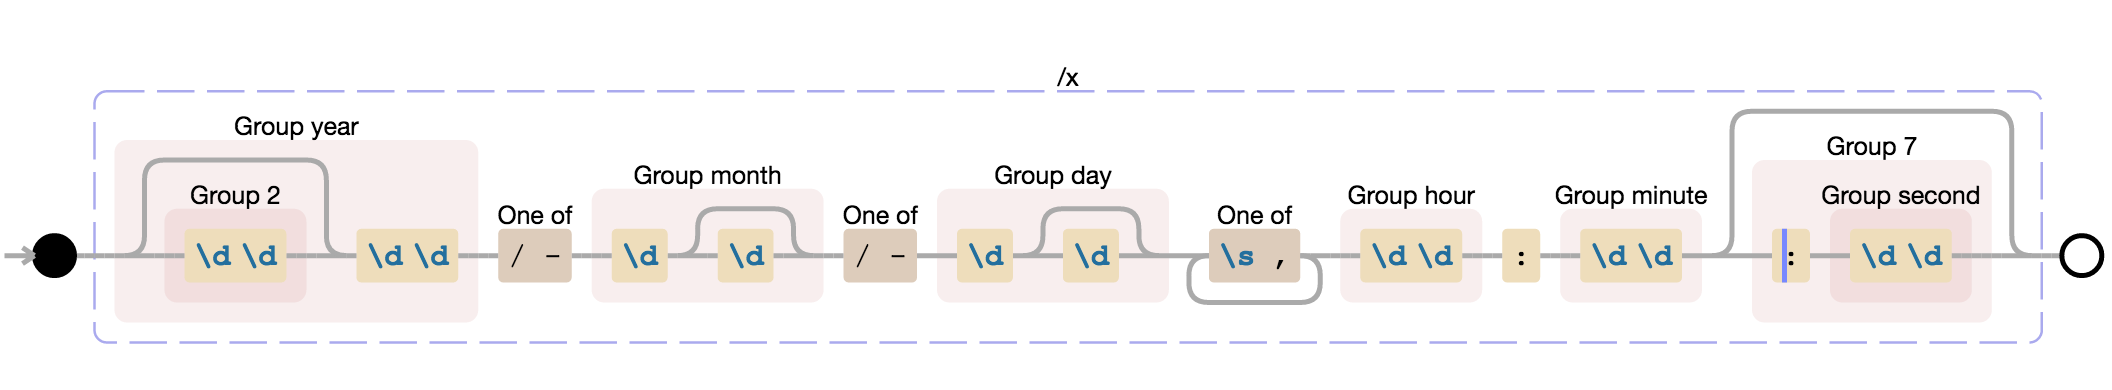
\includegraphics[width=1.0\textwidth]{regex}
\caption{识别发帖时间的正则表达式}
\label{fig:regex}
\end{figure}

如果以发帖时间作为锚节点(Pivot),那么在DOM树中包含发帖时间的最底层的节点,
就定义为锚节点:

\begin{definition}
\label{def:pivot}
$i$是DOM中的一个节点,如果$\vert D_i \vert > 0$且
$\forall j \in descendant(i)$都有$\vert D_j \vert = 0$,
那么$i$就是锚节点
\end{definition}

定义~\ref{def:pivot}~中,$\vert D_i \vert$表示节点$i$的文本中发帖时间的个数,
$descendant(i)$表示$i$的子孙节点集合。

我们可以计算出当前节点所包含的锚节点个数Pivots,
通过Pivots来指导程序发现帖子存在的区域。
类似于算法~\ref{algo:cevc-count}~,这是一个自顶向下的递归计算过程,
Pivots被作为属性,存储在相应节点中。
同样在处理之前,需要从DOM树中移除
\texttt{<script>},\texttt{<style>}和\texttt{comment}。
经过算法countPivots处理之后,我们可以得到一个标注了各个节点Pivots的HTML页面,
如图~\ref{fig:forum-stepinto}~所示。

\begin{figure}[htbp]
\centering
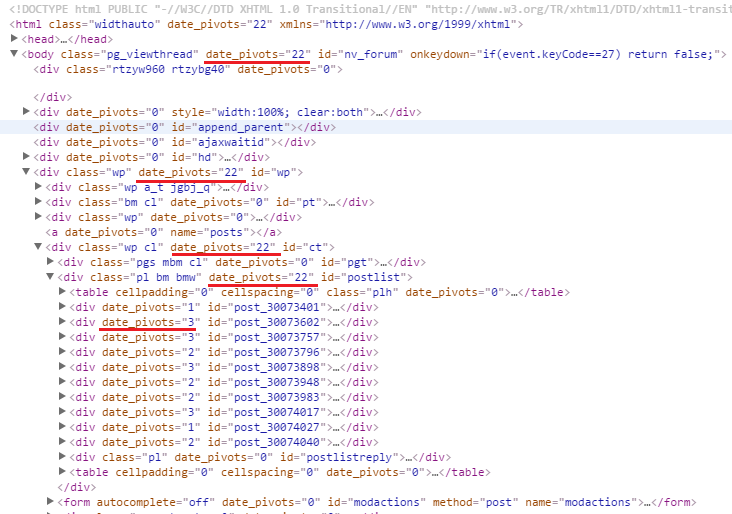
\includegraphics[width=0.9\textwidth]{forum-stepinto}
\caption{时间锚节点示例}
\label{fig:forum-stepinto}
\end{figure}

\subsection{帖子父节点定位方法}
经过大量实例分析,我们发现论坛帖子有一个共同的特点,它们都位于DOM树中同一个父节点之下。
图~\ref{fig:forum-stepinto}~的帖子形式如\texttt{<div\#post\_30073401>},
都位于父节点\texttt{<div\#postlist>}之下。
因为帖子之间是相似的,它们在逻辑地位上是平等的,
论坛网站的服务端程序从数据库中取出数据记录,经过前端模板的渲染最终形成网页,
为了统一对它们进行调整和控制,隶属于同一个父节点是很自然的。

从图~\ref{fig:forum-stepinto}~中可以看到,每个帖子都至少包含一个时间锚节点,
直观地看,时间锚节点密集的区域就是帖子存在的区域。
如果从\texttt{<body>}节点开始,每次都选择时间锚节点最多的子节点深入,
就能定位出一条从\texttt{<body>}通往帖子节点的正确路径,
如图~\ref{fig:forum-stepinto}~中红线标示的节点。
为了描述方便,将这条路径在例~\ref{ex:rmd-mpr}~中列出,其中RMD和MPR在下文中详述。

\begin{example}
\label{ex:rmd-mpr}
RMD和MPR计算过程
\end{example}
\begin{oframed}
\begin{verbatim}
1. <body> Pivots=22 RMD=0 MPR=1
2. <div#wp> Pivots=22 RMD=0 MPR=1
3. <div#ct> Pivots=22 RMD=0 MPR=1
4. <div#postlist> Pivots=22 RMD=0.29 MPR=0.14 帖子的父节点
5. <div#post_30073602> Pivots=3 RMD=0 MPR=1
6. ...
\end{verbatim}
\end{oframed}

每次沿着Pivots最大的子节点不断深入,这个过程不能一直持续下去,
否则会陷入叶节点中,而错失最终的目标节点。
我们定义两个指标,来判断何时停止向下深入的过程。

\begin{definition}
\label{def:rmd}
相对平均偏差(Relative Mean Deviation,RMD)是样本的平均偏差除以样本均值的绝对值:
\begin{equation}
RMD = \frac{\frac{1}{n} \sum_{i=1}^{n} \vert x_i - \bar x \vert}
{\vert \bar x \vert}
\end{equation}
\end{definition}

把同一个父节点下的子节点的时间锚节点个数组成一组样本,去除那些锚节点数为零的样本,
然后计算相对平均偏差RMD,来衡量锚节点在子节点中分布的均匀程度。

因为锚节点属于格式化模板中的一部分,在帖子中分布是较为均匀的,
所以当RMD小于某个阈值时,表明锚节点分布均匀,当前节点下很可能包含一组帖子。
当父节点只有一个子节点包含锚节点时,相对平均偏差为零,这种特殊情况下毫无疑问应当继续深入。
在例~\ref{ex:rmd-mpr}~中,1-3行的RMD都为零,时间锚节点高度集中在一个子节点中。

\begin{definition}
\label{def:mpr}
$i$是DOM树中的一个节点,$i$的最大子节点锚节点占比MPR(Max Pivots Ratio)如下所示,
其中$P_i$表示$i$的锚节点个数,$j$是$i$的子节点:
\begin{equation}
MPR_i = max_{j \in children(i)} \frac{P_j}{P_i}
\end{equation}
\end{definition}

在DOM树中每次向下深入一步,我们认为最大子节点包含了父节点的绝大部分锚节点。
当定义~\ref{def:mpr}~中的MPR低于一个阈值时,
表明最大子节点的锚节点并不足以在父节点中占据统治地位,继续向下深入可能会损失信息。

通过RMD和MPR联合确定停止向下深入的条件,即RMD和MPR都小于各自的阈值时,
向下深入的过程立即终止,当前节点被标记为帖子的父节点。
此时,extract过程负责从当前节点的子节点中筛选出真正的帖子。
这个过程详见算法~\ref{algo:pean-stepinto}~。

\begin{algorithm}[t]
\caption{stepInto(N)}
\label{algo:pean-stepinto}
\KwIn{DOM node N}
\KwOut{Posts}

pivots = $\emptyset$ \;
maxNode = null \;
\For{$C \in N.children()$}{
  \If{$C.pivots > max(pivots)$}{
    maxNode = C \;
  }
  pivots.append(C.pivots) \;
}

\If{maxNode is not null}{
  RMD = computeRMD(pivots) \;
  MPR = max(pivots) / sum(pivots) \;
  \eIf{$pivots.length > 1$ \textbf{and} $RMD < \alpha$ 
    \textbf{and} $MPR < \beta$}{ \label{algo:line:rmd}
    \Return extract(N) \;
  }{
    stepInto(maxNode) \;
  }
}
\end{algorithm}

第~\ref{algo:line:rmd}~行,
在比较RMD和MPR时,还需要确定pivots集合的大小,即包含锚节点的子节点不能只有一个。
在这种情况下单一样本的RMD一定为零,却并不意味着子节点中锚节点分布均匀,
而是锚节点全部集中在一个子节点中,必须继续向下深入。

算法~\ref{algo:pean-stepinto}~能够很快运行结束,因为它至多被递归调用$h$次,
$h$是DOM树的深度,时间复杂度为$O(h)$。

\subsection{候选帖子筛选方法}
在定位了帖子的父节点后,筛选真正的帖子并不是一件简单的工作,
因为帖子的兄弟节点中可能包含很多噪声部分,例如广告、装饰性内容等。
以一篇西陆论坛\footnote{http://club.xilu.com/}的帖子为例,
如图~\ref{fig:forum-noise}~所示,红色实线标示的是真正的帖子,
第一个为楼主发布的主帖,剩下10个为回帖。

这些帖子都位于父节点\texttt{<body>}之下,但\texttt{<body>}之下还有很多非帖子的节点,
\texttt{<div\#BAIDU\_UNION>}是百度联盟提供的广告,
\texttt{<div\#d\_main>}是主帖前后的推荐信息。
如何准确筛选真正的帖子,需要利用帖子和帖子之间DOM树结构的相似性。

\begin{figure}[t]
\centering
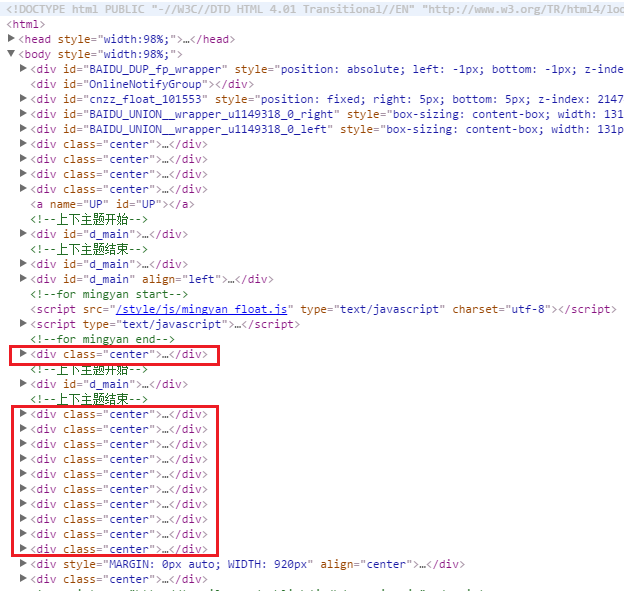
\includegraphics[width=0.9\textwidth]{forum-noise}
\caption{帖子中的噪声}
\label{fig:forum-noise}
\end{figure}

在~\ref{subsec:tree-match}~节的树匹配算法的基础上,可以给出树的相似度定义。

\begin{definition}
\label{def:tree-sim}
已知$M$是两个树$T_1$和$T_2$的匹配,则$T_1$和$T_2$的相似度是:
\begin{equation}
TreeSim(T_1, T_2) = \frac{\vert M \vert}
{(\vert V_1 \vert + \vert V_2 \vert) / 2}
\end{equation}
\end{definition}

其中$\vert M \vert$是$M$中匹配节点的对数,
$\vert V_1 \vert$和$\vert V_2 \vert$分别是$T_1$和$T_2$节点的个数。
从定义~\ref{def:tree-sim}~中可知,树的相似度受树节点规模的影响,
在$\vert M \vert$相同的情况下,
如果$\vert V_1 \vert$或$\vert V_2 \vert$增大就会稀释整个相似度。

我们从图~\ref{fig:post-match}~中的例子分析,
这两个子树代表两个帖子,虚线连接的是相互匹配的节点。
帖子第一层子节点中,代表发帖时间和发帖内容的节点都能够相互匹配,
但灰色节点标志的用户生成内容却不能匹配。
论坛帖子有别于商品展示信息,它的内容由用户生成(UGC),
具有很高的自由度,因此体现出高度差异化和多样性。
左边帖子直接包含文本和换行标签\texttt{<br>},
右边帖子则通过\texttt{<p>}包裹文本,并提供了一张图片\texttt{<img>}。

\begin{figure}[htbp]
\centering
\begin{tikzpicture}[
level 1/.style={sibling distance=2cm},
level 2/.style={sibling distance=2cm},
level 3/.style={sibling distance=1cm},
tag/.style={circle, draw},
leaf/.style={rectangle, draw, text width=2cm},
gray/.style={fill=gray},
]
\node[tag](A1){div}
  child{node[tag](B1){div}
    child{node[leaf]{\footnotesize 2016-02-16}}
  }
  child{node[tag](C1){div}}
  child{node[tag](D1){div}
    child{node[leaf, gray]{\footnotesize There is something}}
    child{node[tag, gray]{\footnotesize br}}
  }
;
\node[tag, right=8cm of A1](A2){div}
  child{node[tag](B2){div}
    child{node[leaf]{\footnotesize 2016-03-10}}
  }
  child{node[tag](C2){div}}
  child{node[tag](D2){div}
    child{node[tag, gray]{\footnotesize p}
      child{node[leaf, gray]{\footnotesize The photo is amazing!}}
    }
    child{node[tag, gray]{\footnotesize img}}
  }
;
\draw [dashed, thick, ->](A1) to [bend left](A2);
\draw [dashed, thick, ->](B1) to [bend left](B2);
\draw [dashed, thick, ->](C1) to [bend left](C2);
\draw [dashed, thick, ->](D1) to [bend left](D2);
\end{tikzpicture}
\caption{帖子的匹配}
\label{fig:post-match}
\end{figure}

如果直接使用定义~\ref{def:tree-sim}~的树相似度计算,
就会被高度自由的UGC节点干扰,使两个帖子原本应该很高的相似度降低,最后被认为不相似而遗漏。
和字符串的最长公共子序列类似,最大匹配节点数反映了两个树之间“重合”部分的大小。
虽然UGC内容带来的结构、形式差异会导致帖子间相似度参差不齐,
但相互之间能够匹配的最大节点数却比较稳定,可以利用这个“重合”部分来度量相似性。

从候选子节点中筛选真正帖子的过程extract,如算法~\ref{algo:pean-extract}~所示。
算法~\ref{algo:pean-stepinto}~中选定的maxNode在这里被当做基准节点,
其它至少包含一个锚节点的兄弟节点一一与之进行树匹配计算,
然后以节点作为key、最大匹配节点数作为value存储在一个map数据结构中。

基准节点maxNode被认定为帖子,output过程将其内容输出。
其它节点按照和基准节点之间重合部分的大小,从高到低排列,
虽然它们彼此的相似度可能参差不齐,但重合度却比较稳定。
按照这个顺序遍历最大匹配节点个数,如果发现某个最大匹配节点数低于前者的一半,
就认为筛选结束,该节点之前的都属于目标帖子,而放弃之后重合度太低的节点。

\begin{algorithm}[t]
\caption{extract(N, maxNode)}
\label{algo:pean-extract}
\KwIn{DOM node N, maxNode}
\KwOut{Posts}

mappings = $\emptyset$ \;
\For{$C \in N.children()$}{
  \If{$C \neq maxNode$ \textbf{and} $C.pivots > 0$}{
    mappings[C] = treeMatch(C, maxNode) \;
  }
}

output(maxNode) \;
lastNum = 0 \;
\For{$C \in$ mappings ordered from high to low}{
  \If{$mappings[C] < lastNum / 2$}{
    \textbf{break} \;
  }
  lastNum = mappings[C] \;
  output(C) \;
}
\end{algorithm}

记候选帖子数量为$m$,每个帖子的平均节点数为$n$。
算法~\ref{algo:pean-extract}~的运算分为两部分:
\begin{enumerate}
\item 首先是基准节点和候选帖子节点之间的树匹配过程,
因为treeMatch的复杂度为$O(n^2)$,所以其复杂度为$O(mn^2)$。
\item 另一部分是对候选帖子的排序、遍历过程,
排序复杂度为$O(m\log m)$,所以其复杂度为$O(m\log m)$。
\end{enumerate}

一般情况下,由于论坛结构和UGC内容日趋丰富,再加上分页对单篇网页帖子数量的限制,
候选帖子数量$m$小于帖子的平均节点数$n$,自然有$n^2 > \log m$,
算法~\ref{algo:pean-extract}~extract的总体时间复杂度为$O(mn^2)$。

\subsection{算法实现概述}
面对HTML网页中普遍存在的代码错误,例如缺失结束标签、使用非标准的标签和错误的嵌套等,
这里使用Python第三方库BeautifulSoup来尽可能纠正这些错误。
BeautifulSoup是一个可以从HTML或XML文件中提取数据的Python库,
它为操作DOM提供了一套方便的接口,底层调用lxml等具体的解析器,
能够处理有代码错误的网页。

PEAN需要从HTML文档中抽取发帖时间,
所使用的正则表达式在~\ref{subsec:anchor}~节已经描述过。


\section{论坛帖子抽取实验}
\label{sec:pean-experiment}

\subsection{帖子抽取评价指标}
为了验证算法的抽取效果,我们定义标准评价指标准确率Precision、召回率Recall和
F\textsubscript{1}。
通过比较算法抽取的帖子集合$e$和金标准的帖子集合$g$,Precision、Recall和
F\textsubscript{1}可以如下计算:

\begin{equation}
P = \frac{\vert e \cap g \vert}{\vert e \vert}, 
R = \frac{\vert e \cap g \vert}{\vert g \vert}
\end{equation}
\begin{equation}
F_1 = \frac{2 \times P \times R}{P + R}
\end{equation}

在计算一个网站或一个算法整体的评价指标时,是将每个单独网页的正确抽取帖子数累加计算的,
而不是简单计算平均值,Precision如下所示,Recall和F\textsubscript{1}的计算类似。

\begin{equation}
P = \frac{\sum \vert e_i \cap g_i \vert}{\sum \vert e_i \vert}
\end{equation}

\subsection{论坛数据集}
为了验证帖子抽取算法在实际中文论坛上的抽取效果,
我们从知名的网址导航网站hao123\footnote{https://www.hao123.com/}
和360导航\footnote{https://hao.360.cn/}
中任意选取了20个知名的论坛网站作为测试对象,如表~\ref{tbl:forum-dataset}~所示。
从采集的网页中,去除失效的、没有回帖的网页,
总计有效网页973个,平均每个网站50个以内。

\begin{table}[t]
\caption{论坛数据集}
\label{tbl:forum-dataset}
\vspace{0.5em}\centering\wuhao
\begin{tabular}{llll}
\toprule[1.5pt]
编号 & 论坛名称 & 论坛代码 & 网址 \\
\midrule[1pt]
1 & 网易论坛 & 163 & http://bbs.163.com/ \\
2 & 360安全社区 & 360safe & http://bbs.360safe.com/ \\
3 & 55BBS论坛 & 55bbs & http://bbs.55bbs.com/ \\
4 & 腾讯论坛 & qq & http://bbs.ent.qq.com/ \\
5 & 环球论坛 & huanqiu & http://bbs.huanqiu.com/ \\
6 & 春秋社区 & ichunqiu & http://bbs.ichunqiu.com/ \\
7 & 卡饭论坛 & kafan & http://bbs.kafan.cn/ \\
8 & 远景论坛 & pcbeta & http://bbs.pcbeta.com/ \\
9 & 看雪学院 & pediy & http://bbs.pediy.com/ \\
10 & 瑞丽论坛 & rayli & http://bbs.rayli.com.cn/ \\
11 & 天涯社区 & tianya & http://bbs.tianya.cn/ \\
12 & 铁血论坛 & tiexue & http://bbs.tiexue.net/ \\
13 & 精睿 & vc52 & http://bbs.vc52.cn/ \\
14 & 华声论坛 & voc & http://bbs.voc.com.cn/ \\
15 & 中华网论坛 & china & http://club.china.com/ \\
16 & 新浪论坛 & sina & http://club.history.sina.com.cn/ \\
17 & 凯迪社区 & kdnet & http://club.kdnet.net/ \\
18 & 宽带山 & pchome & http://club.pchome.net/ \\
19 & 西陆论坛 & xilu & http://club.xilu.com/ \\
20 & 泡泡俱乐部 & pcpop & http://pop.pcpop.com/ \\
\bottomrule[1.5pt]
\end{tabular}
\end{table}

数据的采集和标注都需要消耗很多的精力,为了节省人力成本,
我们通过构建特定论坛的包装器来解决这个问题。
如例~\ref{ex:forum-wrapper}~所示,
FORUM是Python的字典结构,以key-value对的形式存储各个论坛的详细配置。

以网易论坛为例,采集程序从板块地址\url{http://bbs.news.163.com/}入手,
得到某个板块的网页,然后通过thread的CSS选择符定位每个thread的url。
选择符\texttt{ul.rankList a[href]}的含义是,
选择所有\texttt{<ul class='rankList'>}标签下的,
有\texttt{href}属性的\texttt{<a>}标签。
同理,通过帖子的CSS选择符可以标注真正的帖子,供后续实验分析。

\begin{example}
\label{ex:forum-wrapper}
论坛包装器示例
\end{example}
\begin{oframed}
\begin{verbatim}
FORUM = {
  '163': {
    'name': '网易论坛',                   # 论坛名称
    'home': 'http://bbs.163.com/',        # 论坛主页地址
    'board': 'http://bbs.news.163.com/',  # 论坛板块地址
    'thread': ['ul.rankList a[href]'],    # 论坛thread的CSS选择符 
    'post': ['div.tie-item'],             # 论坛帖子的CSS选择符
  }}
\end{verbatim}
\end{oframed}

这里的CSS选择符可以是一个列表,包含不止一个选择符,以应对更负责的情况。
例如在凯迪社区的配置中,帖子既可能是\texttt{div.reply-box},
也可能是\texttt{div.posted-box-add},对应主帖和后续跟帖。

\subsection{实验过程和结果分析}

实验环境为一台MacBook Pro(2 GHz Intel Core i7处理器,8G内存,256G SSD),
详细的实验过程如下:
\begin{enumerate}
\item 将下载的论坛原始HTML网页统一保存在本地文件夹,
以“网站名-URL的MD5.html”的形式命名。
\item 分别用Python实现MiBAT算法和PEAN算法,并提供统一的调用接口。
输入HTML源文件,算法在内存中构建DOM树,对每个抽取到的帖子,
都在相应的DOM树标签上追加一个自定义属性,例如\texttt{marked-by-MiBAT}。
全部处理完毕后,算法将DOM树重新序列化为HTML源文件返回。
\item 编写测试脚本,首先对待测试的论坛网页进行预处理。
通过例~\ref{ex:forum-wrapper}~中人工编写的包装器,
对每一个金标准指定的帖子,在相应的DOM树标签上追加一个自定义属性,
\texttt{this-is-real-post}。
\item 然后测试脚本先后调用MiBAT和PEAN算法,得到处理后的DOM树,
统计既有\texttt{marked-by-MiBAT}属性,
又有\texttt{this-is-real-post}属性的DOM树标签个数,来计算MiBAT算法的性能指标。
通过这种在DOM树中追加自定义属性的方式,能够方便地统计不同算法的抽取效果。
\item 实验结果以日志的形式保存在文件中,便于后续整理。
\end{enumerate}

在20个论坛构成的数据集上对MiBAT和PEAN算法分别进行评估,
实验结果如表~\ref{tbl:pean-all}~所示,
列出了精确率、召回率和F\textsubscript{1}三项指标。
每一行代表一个网站的测试结果,粗体标示的是MiBAT和PEAN在F\textsubscript{1}上的优胜者。

从表~\ref{tbl:pean-all}~中可以看出,在不同论坛网站上,两种算法各有优劣。
MiBAT的总体精确率较高,达到了99.6\%,高于PEAN的98.3\%,
但却牺牲了召回率,导致总体F\textsubscript{1}只有84.6\%,
比PEAN的94.7\%低了很多。
实验结果表明,PEAN相比于MiBAT在召回率指标上有大幅度提升,
总体F\textsubscript{1}指标也优于MiBAT。

\begin{table}[t]
\caption{MiBAT和PEAN在论坛数据集上的对比结果}
\label{tbl:pean-all}
\vspace{0.5em}\centering\wuhao
\begin{tabular}{lllllll}
\toprule[1.5pt]
论坛名称 & MiBAT-P & MiBAT-R & MiBAT-F\textsubscript{1} &
PEAN-P & PEAN-R & PEAN-F\textsubscript{1} \\
\midrule[1pt]
网易论坛 & 100.0\% & 97.0\% & 98.5\% & 100.0\% & 100.0\% & \textbf{100.0\%} \\
360安全社区 & 100.0\% & 63.4\% & 77.6\% & 100.0\% & 97.5\% & \textbf{98.7\%} \\ 
环球论坛 & 100.0\% & 48.8\% & 65.6\% & 100.0\% & 97.7\% & \textbf{98.8\%} \\
春秋社区 & 100.0\% & 62.3\% & 76.8\% & 100.0\% & 100.0\% & \textbf{100.0\%} \\
卡饭论坛 & 100.0\% & 78.9\% & 88.2\% & 100.0\% & 95.3\% & \textbf{97.6\%} \\
远景论坛 & 100.0\% & 99.6\% & \textbf{99.8\%} & 100.0\% & 97.9\% & 98.9\% \\
看雪学院 & 100.0\% & 98.8\% & \textbf{99.4\%} & 100.0\% & 97.5\% & 98.8\% \\
腾讯论坛 & 100.0\% & 39.3\% & 56.5\% & 100.0\% & 92.0\% & \textbf{95.8\%} \\
瑞丽论坛 & 100.0\% & 100.0\% & \textbf{100.0\%} & 62.5\% & 67.7\% & 65.0\% \\
新浪论坛 & 100.0\% & 99.7\% & \textbf{99.8\%} & 100.0\% & 92.9\% & 96.3\% \\
天涯社区 & 100.0\% & 98.6\% & 99.3\% & 100.0\% & 100.0\% & \textbf{100.0\%} \\
铁血论坛 & 83.1\% & 7.7\% & 14.0\% & 100.0\% & 89.3\% & \textbf{94.3\%} \\
精睿 & 100.0\% & 86.4\% & 92.7\% & 100.0\% & 98.6\% & \textbf{99.3\%} \\
华声论坛 & 100.0\% & 94.7\% & \textbf{97.3\%} & 100.0\% & 89.4\% & 94.4\% \\
中华网论坛 & 100.0\% & 88.5\% & \textbf{93.9\%} & 93.5\% & 13.9\% & 24.2\% \\
凯迪社区 & 100.0\% & 87.5\% & \textbf{93.3\%} & 100.0\% & 83.0\% & 90.7\% \\
宽带山 & 99.8\% & 98.3\% & \textbf{99.1\%} & 99.8\% & 98.0\% & 98.9\% \\
西陆论坛 & 100.0\% & 61.0\% & \textbf{75.8\%} & 100.0\% & 53.5\% & 69.7\% \\
泡泡俱乐部 & 100.0\% & 76.4\% & 86.6\% & 100.0\% & 95.0\% & \textbf{97.4\%} \\ 
55BBS & 100.0\% & 93.0\% & \textbf{96.4\%} & 92.6\% & 90.7\% & 91.6\% \\
总计 & 99.6\% & 73.5\% & 84.6\% & 98.3\% & 91.3\% & \textbf{94.7\%} \\
\bottomrule[1.5pt]
\end{tabular}
\end{table}

MiBAT在树相似度计算过程中,尽可能选择隶属于格式化模板的一部分节点进行比较,
而不是将所有节点全部考虑进去。
最佳情况是,tree fragment选择函数直接选取了树的模板部分,但这难以做到。
作者给出了一个近似,即锚节点和锚节点的兄弟节点,
认为这部分节点在不同帖子中结构相对固定,有利于相似度的计算。

但在实验结果中发现,随着近年来论坛页面复杂程度的提高,
帖子和帖子之间的差异性越来越大。
许多帖子在锚节点和锚节点的兄弟节点这个层面上出现了不同,
虽然不匹配的节点\textbf{绝对数量}并不多,
但在相似度计算中真正起关键作用的\textbf{相对比例}却足够大,
所以导致整体相似度大幅度降低。

例如图~\ref{fig:forum-compare}~的一篇
360安全社区\footnote{http://bbs.360safe.com}所示,
红色矩形标示的是MiBAT所抽取的帖子,网页中的第一个帖子被遗漏了。
分析原因发现,蓝色矩形标示的是锚节点,
但后面的两个帖子中出现了对发帖的引用(红色椭圆),干扰了锚节点和兄弟节点结构的稳定性,
算法倾向于选择相似度更高的结果。

\begin{figure}[htbp]
\centering
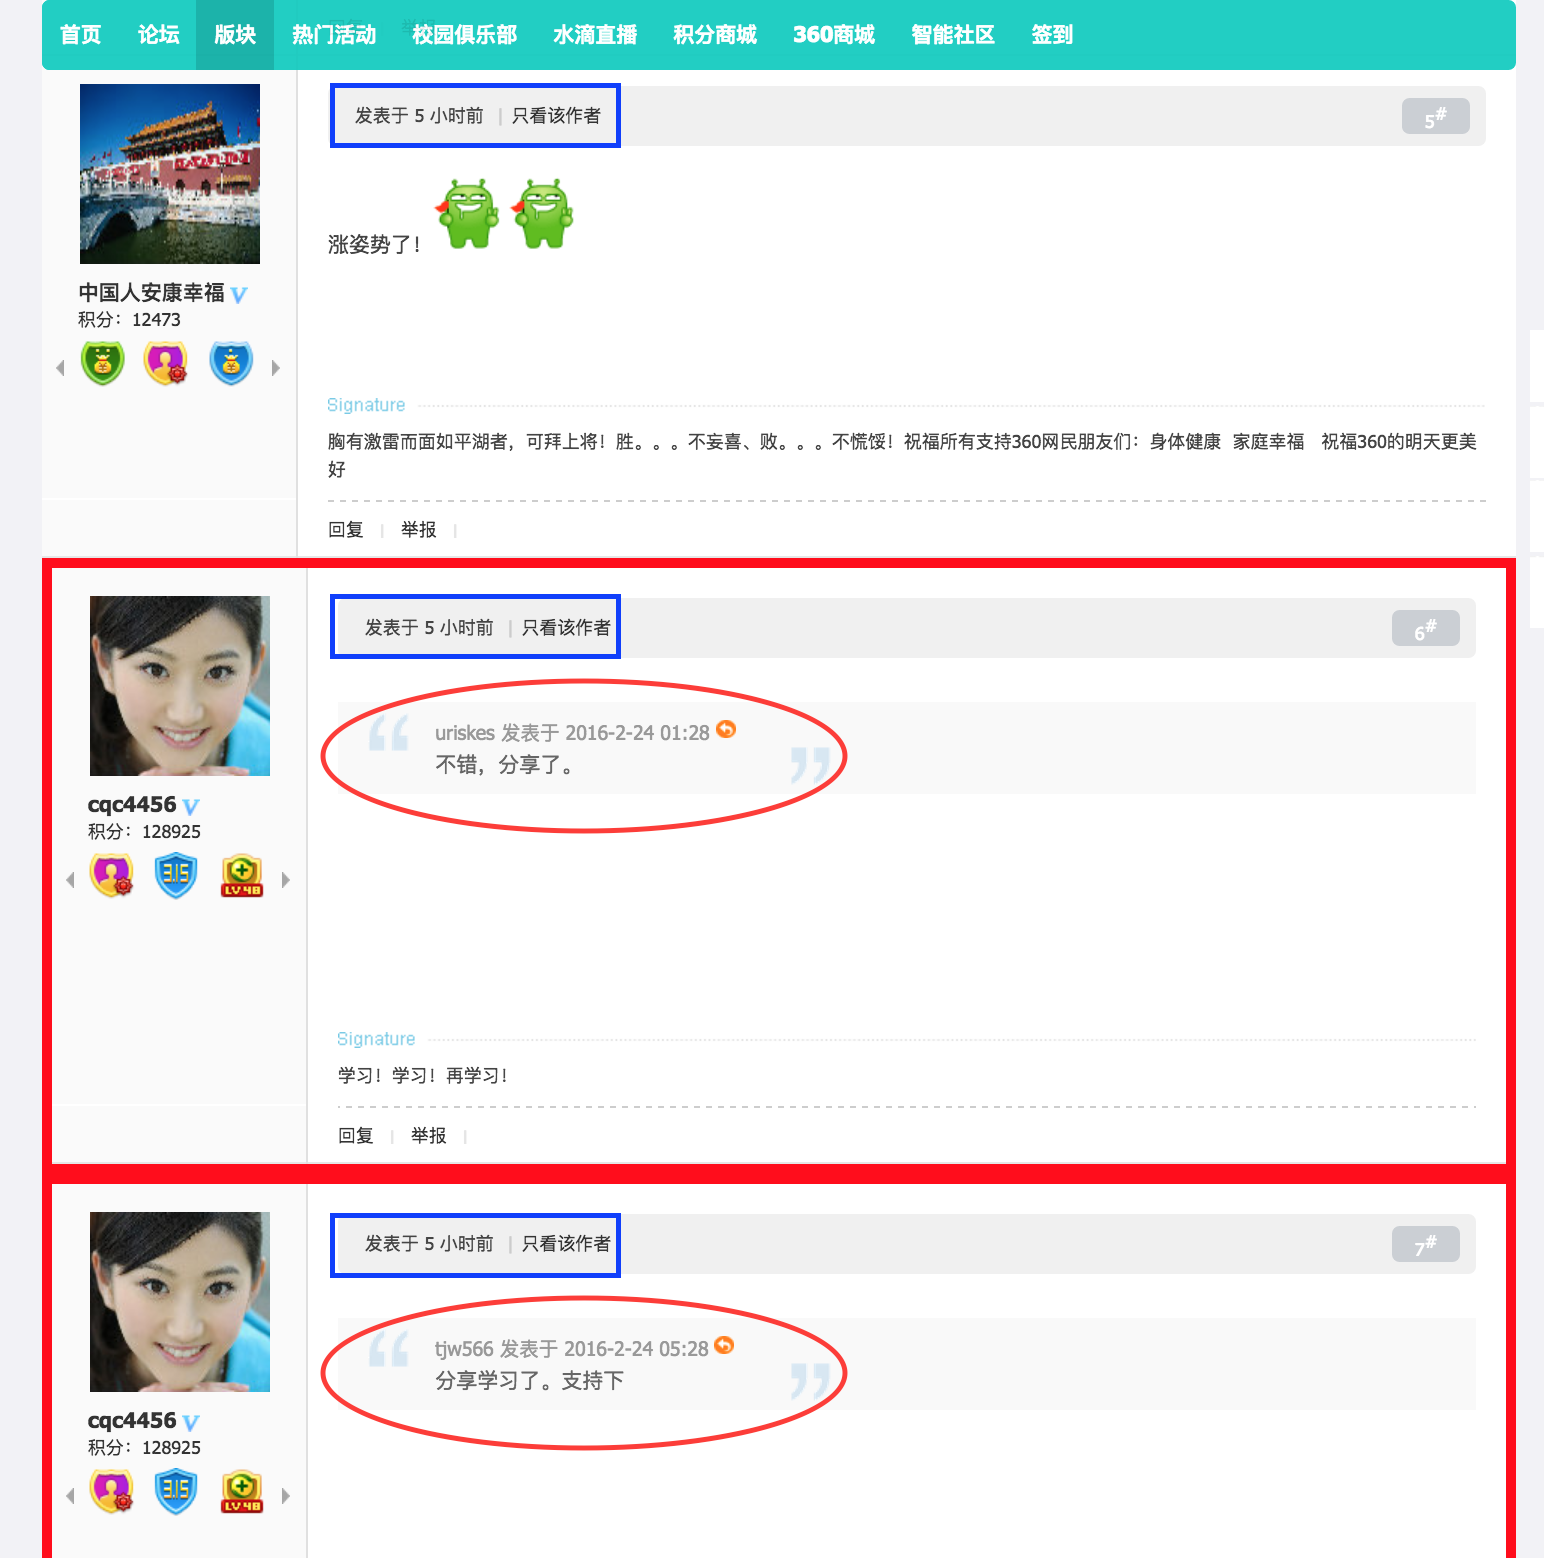
\includegraphics[width=0.9\textwidth,height=0.45\textheight]{forum-compare}
\caption{锚节点及其兄弟节点的差异性}
\label{fig:forum-compare}
\end{figure}

\begin{figure}[htbp]
\centering
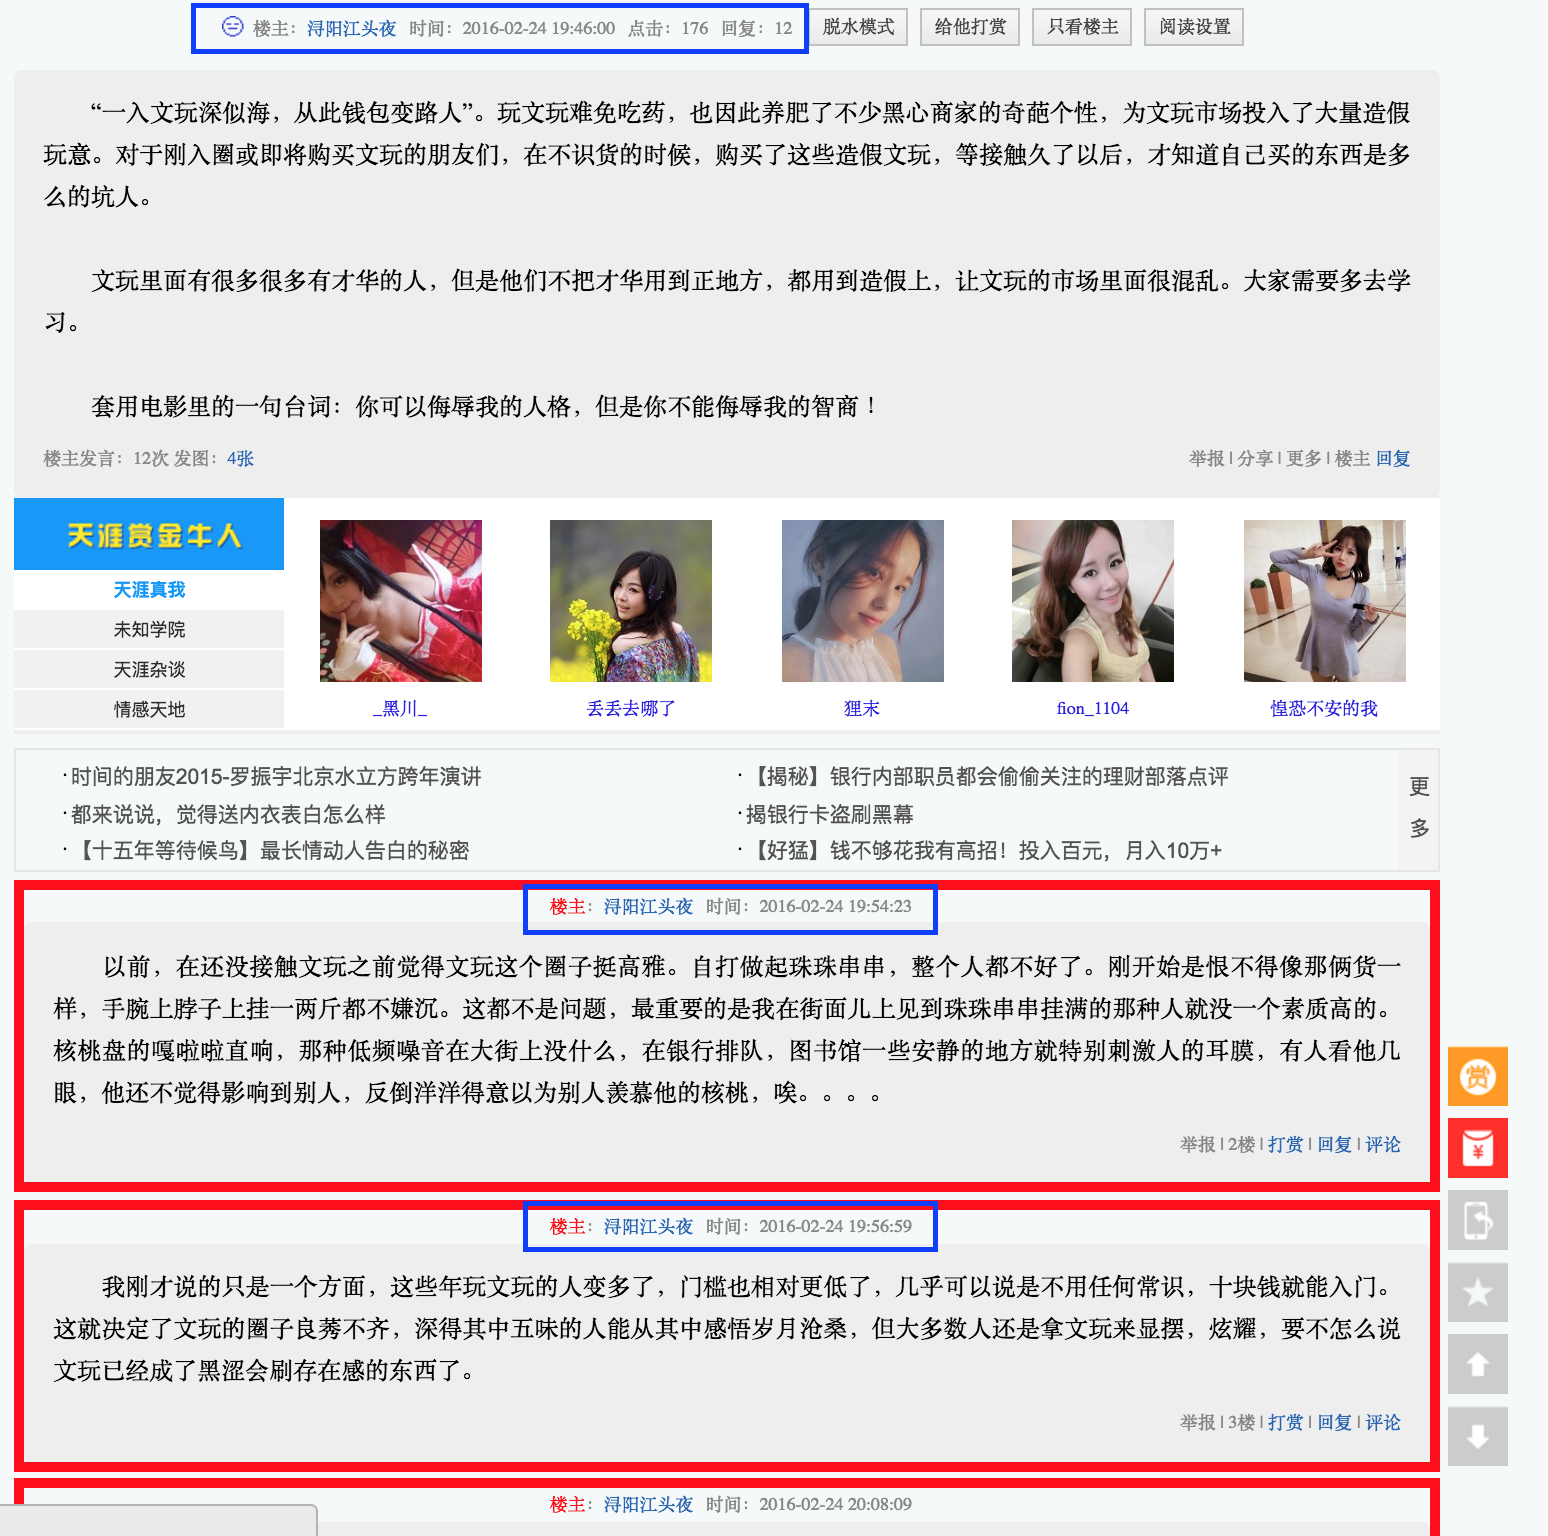
\includegraphics[width=0.9\textwidth,height=0.45\textheight]{forum-compare2}
\caption{楼主发帖和其它帖子的区别}
\label{fig:forum-compare2}
\end{figure}

还有一种情况,在论坛页面的楼主发帖(第一个帖子)中,
形式结构和后续跟帖在锚节点层面上有较大不同。
如图~\ref{fig:forum-compare2}~的一篇
天涯社区\footnote{http://bbs.tianya.cn}所示,蓝色矩形标示的锚节点中,
楼主发帖的锚节点包含额外的点击、回复信息,导致依赖锚节点及其兄弟节点的相似度匹配失效。

PEAN算法直接计算两个候选帖子中最大匹配节点个数,
来衡量“重合”部分的大小,避免了片面选择Tree Fragment带来的不稳定性,
在实验中取得了更好的效果。

\section{本章小结}
\label{sec:pean-conclusion}

本章研究自动化的论坛帖子抽取技术,
首先介绍了对比算法MiBAT(基于锚点树的数据记录抽取算法)的原理和实现细节,
针对其存在的问题做出改进,提出一种基于锚节点的论坛帖子抽取算法PEAN。
该算法利用了论坛帖子中普遍存在的发帖时间作为锚节点,
利用锚节点的分布确定一组帖子的位置,然后通过树匹配算法衡量相似性,筛选出真正的帖子。
最后从知名的中文论坛网站上采集网页进行实验。
实验结果表明PEAN相比于MiBAT在召回率指标上有大幅度提升,
平均94.7\%的F\textsubscript{1}-measure也优于MiBAT。
